\documentclass{article}

% Language setting
% Replace `english' with e.g. `spanish' to change the document language
\usepackage[english]{babel}
\usepackage{fontawesome5}
% Set page size and margins
% Replace `letterpaper' with `a4paper' for UK/EU standard size
\usepackage[letterpaper,top=2cm,bottom=2cm,left=3cm,right=3cm,marginparwidth=1.75cm]{geometry}

% Useful packages
\usepackage{amsmath}
\usepackage{graphicx}
\usepackage[colorlinks=true, allcolors=blue]{hyperref}

\usepackage{booktabs}
\usepackage{siunitx}

\title{Problem Set 7}
\author{JaeSeok Oh}

\begin{document}
	\maketitle
	

\section*{Imputing Missing Data Practice}
\subsection*{Q6.}
	\begin{itemize}
		\item \textit{logwages} are missing at approximately 25\% $\left( =  \displaystyle\frac{560}{1669} * 100 \right)$ of the total number of observations.  Since wages cannot be negative, it would not be the case of MNAR.
		\begin{table}[h]
			\centering
			\caption{Data Summary}
			\begin{tabular}[t]{lrrrrrrrrrr}\toprule  & mean & SD & Min & Max & Median & P0 & P25 & P50 & P75 & P100\\\midrule
				logwage &  & \num{0.39} & \num{0.00} & \num{2.26} & \num{1.66} & \num{0.00} & \num{1.36} & \num{1.66} & \num{1.94} & \num{2.26}\\hgc & \num{13.10} & \num{2.52} & \num{0.00} & \num{18.00} & \num{12.00} & \num{0.00} & \num{12.00} & \num{12.00} & \num{15.00} & \num{18.00}\\tenure & \num{5.97} & \num{5.51} & \num{0.00} & \num{25.92} & \num{3.75} & \num{0.00} & \num{1.58} & \num{3.75} & \num{9.33} & \num{25.92}\\age & \num{39.15} & \num{3.06} & \num{34.00} & \num{46.00} & \num{39.00} & \num{34.00} & \num{36.00} & \num{39.00} & \num{42.00} & \num{46.00}\\\bottomrule
			\end{tabular}
		\end{table}
		\begin{table}[h]
			\centering
			\caption{Missing Data Details}
			\begin{tabular}[t]{ccccccccccc}
				\toprule
				& \multicolumn{2}{c}{college} && \multicolumn{2}{c}{married} && \multicolumn{4}{c}{Intersection} \\\cline{2-3} \cline{5-6} \cline{8-11}
				& grad & ngrad & & mar & sin && grd\&mar & ngrd\&mar & grd\&sin &ngrd\&sin  \\\midrule
				Missing &273 & 287& & 339 & 221 &&164&175&109&112 \\
				Complete & 257 & 1412 && 1092 & 577 &&179&913&78&499 \\\bottomrule
			\end{tabular}
		\end{table}
		\item In Table 2, we can see the ratio of individual characteristics(college and marriage) of \textit{logwages} missing. Most wage values are from non-college graduate individuals, as well as married individuals. However, the ratio of missing values is high on graduate individuals and single individuals.
		\item In detail, I tabled the counts of the intersection terms between \textit{married} and \textit{college}. It is noticeable that those who graduated from college missed their wage values. Moreover, the ratio is much higher for the individuals who graduated and single.
		\begin{figure}[h]
			\centering
			\caption{}
			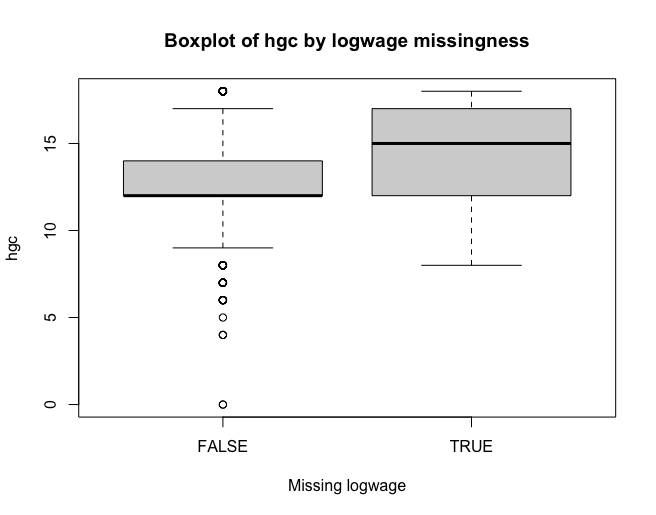
\includegraphics[width = 100mm]{hgc_boxplot.png}
		\end{figure}
		\item I also conducted the comparison of \textit{hgc} between missing and complete \textit{logwage}. As in Figure 1, \textit{hgcs}, missing \textit{logwages}(right side), have a higher mean and wider range of values. This result is consistent with the previous comment on that missings occurred more frequently in graduate individuals. 
		\item Therefore, to make a conclusion that the missings are MAR cases is reasonable, even though the reason is not clear.
	\end{itemize}

\subsection*{Q7.}
	\begin{itemize}
		\item Table 3 shows four different imputation method results by running linear regression:
		\begin{equation}
			logwage_{i} = \beta_{0} + \beta_{1}hgc_{i} + \beta_{2}college_{i} + \beta_{3}tenure_{i} + \beta_{4}tenure^{2} + \beta_{5}age_{i} + \beta_{6}married_{i} + \varepsilon_{i}
		\end{equation}
		\begin{table}[h]
			\centering
			\caption{Regression Results}
			\begin{tabular}[t]{lcccc}\toprule  & Raw & Mean Imp & Predicted Imp & Multiple Imp\\\midrule(Intercept) & \num{0.534}*** & \num{0.708}*** & \num{0.534}*** & \num{0.606}***\\ & (\num{0.146}) & (\num{0.116}) & (\num{0.112}) & (\num{0.159})\\hgc & \num{0.062}*** & \num{0.050}*** & \num{0.062}*** & \num{0.061}***\\ & (\num{0.005}) & (\num{0.004}) & (\num{0.004}) & \vphantom{1} (\num{0.006})\\college & \num{0.145}*** & \num{0.168}*** & \num{0.145}*** & \num{0.125}***\\ & (\num{0.034}) & (\num{0.026}) & (\num{0.025}) & (\num{0.031})\\tenure & \num{0.050}*** & \num{0.038}*** & \num{0.050}*** & \num{0.041}***\\ & (\num{0.005}) & (\num{0.004}) & (\num{0.004}) & (\num{0.006})\\ tenure$^{2}$ & \num{-0.002}*** & \num{-0.001}*** & \num{-0.002}*** & \num{-0.001}**\\ & (\num{0.000}) & (\num{0.000}) & (\num{0.000}) & (\num{0.000})\\age & \num{0.000} & \num{0.000} & \num{0.000} & \num{0.000}\\ & (\num{0.003}) & (\num{0.002}) & (\num{0.002}) & (\num{0.003})\\married & \num{-0.022} & \num{-0.027}* & \num{-0.022}+ & \num{-0.018}\\ & (\num{0.018}) & (\num{0.014}) & (\num{0.013}) & (\num{0.015})\\\midrule
				Num.Obs. & \num{1669} & \num{2229} & \num{2229} & \num{2229}\\R2 & \num{0.208} & \num{0.147} & \num{0.277} & \num{0.223}\\\bottomrule\multicolumn{5}{l}{\rule{0pt}{1em}+ p $<$ 0.1, * p $<$ 0.05, ** p $<$ 0.01, *** p $<$ 0.001}\\
			\end{tabular}
		\end{table}
		\item Column 1 is the regression result from the data set after dropping the missing \textit{logwages}, while the others are the estimates after filling out the missing values by the several imputation methods: (2) mean, (3) predicted from the result of Column 1, and (4) multiple imputation by using \textit{mice} R package.
		\item Compared to the true value of $ \widehat{\beta}_{1} = 0.093 $, all of them are down-ward estimated. It can apparently be explained by the pattern of missings: \textit{logwages} of higher \textit{hgc} are missing. This pattern should lead the estimates in terms of \textit{hgc} to be lowered. We can see the `mean imputation method' do the worst work because this might not be able to capture the \textit{hgcs}' differences on the missing values.
		\item $ \widehat{\beta}_{1} $ is estimated most closely in the first and the third regressions -- these two are almost the same. This is evident because the data used in the third regression model is derived from the results of the first estimation with lower standard errors. Thus, the veracity of the predicted imputation depends on the validity of the first regression model. In contrast, the fourth regression result of  $ \beta_{1} $ seems a concrete reference to recover the true $ \beta_{1} $ because it generates the values in random. However, in this case, we know that there is a skewness in the distribution of missing values among graduate and single individuals or higher mean \textit{hgc}, which is not in completely random.
		\item Therefore, if one was able to figure out whether MCAR, MAR, or MNAR, one could choose the method. In the case of completely at random, multiple imputation (fourth estimates) might be better due to the uncertainty of missing pattern, while in the case of just at random, predicted imputation might reflect the differences(statistical logic or observed) better.
	\end{itemize}
	
\subsection*{Q8.}
\begin{itemize}
	\item I am still using the data set I downloaded from \textbf{`kaggle'}. For me, it is required to look at firstly the literature of the sequential auction. And then, I could make a further decision to implement web-scrape or think of the other way to explore significant implications.
	\item Now, I am modeling the data as `long-panel' data with a time trend to capture the price pattern overtime.
\end{itemize}

		
		
		

\end{document}